\subsection{The development environment}
The virtual keyboard took far more time than I had initially anticipated. It required me to delve into the installation process for Komodo as I had no knowledge of how to attach software to Komodo. When browsing through the set-up folder and bash script for Komodo, I found the Jimulator plug-ins which my tutor had pointed me in the direction of. These plug-ins act as event handlers for the ARM chip. They can respond to things like SVC commands, memory reads and memory writes. The useful thing about these plugins is that they can also affect the chip in various ways by causing interrupt signals and writing data to specific registers. This is essentially how all of the input and output was handled in COMP151111. In this course the students would make a SVC\_0 call which Jimulator would intercept, and then output R0 to the built-in terminal. In much the same way a call to SVC\_1 would be intercepted by Jimulator causing a read from the terminal into R0. The scripts included in the default installation of komodo also included a virtual keypad, a timer, and a virtual screen. I had used the screen and keypad before but I wanted more keys for the keypad, in order to make inputting letters easier. Naturally, the keypad plug-in became my reference for creating a plug-in as it was the closest in purpose for what I wanted to achieve. 

I determined from the keypad plug-in that the actual interface seen by the user was a simple python script executed during komodo's start-up. This script parsed an XML file which defined the layout of the keypad. This script then also passed the states of the buttons to a piece of shared memory. This shared memory was then attached in the plug-in script and when ever a read was made to the keypads location, the plug-in would intercept it and update it according to the contents of the shared memory. The last bit of knowledge I needed was how to compile the plug-in, into something jimulator could actually work with. From reading the make file I determined that the code had to bed compiled with the --shared flag to compile a shared object and the fPIC flag to indicate it is a library and may be executed from anywhere so its jumps need to be calculated relatively rather than absolutely.
\subsection{Design}
\subsubsection{Virtual Keyboard Hardware Interfaces}
The virtual keyboard design is very similar in concept to the virtual keypad explained above. However it differs hugely in how it appears as a peripheral in the ARM environment. The keypad used in the COMP22712 labs appears as a single byte, in which bits 7-5 are set in turn to allow bits 3 - 0 to be scanned into. This set-up requires the system to scan they keyboard themselves and denounce the result. While this is also a possible protocol to implement with the larger keyboard I built, I felt it made more sense to have the virtual keyboard appear as 3 bytes, one to trigger the data change, one to represent an ascii character, one to represent the direction of the button interaction (pushed or unpushed).

The advantages of handling the keyboard this way are that I don't have to have as much processing on the ARM side. This is very helpful as the code required to scan a virtual keyboard can be quite cumbersome and time consuming. This interface also allows me to mimic modern hardware, which would send ascii codes, rather than requiring the processor to manage the IO more manually. 
\subsubsection{Keyboard Design}
I used the python library glade to model the keyboard. Unfortunately, lots of these buttons are there for appearance sake only, as this keyboard does not implement a full ASCII character set. I chose to do this as I felt the time to benefit ratio did not warrant spending more time on this. While I could have implemented more control characters, I would be highly unlikely to use them so I felt it would be wasted time. 

\begin{figure}[ht!]
	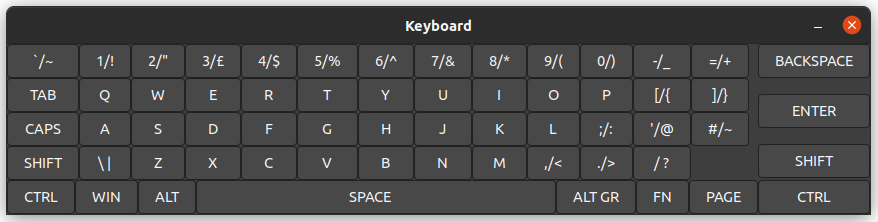
\includegraphics[width=\linewidth]{figures/keyboard.png}
	\caption{The final design of the virtual keyboard}
	\label{fig:keyboard}
\end{figure} 
 
I managed to implement working characters from ASCII 0x20 to 0x7F as well as working caps-lock, shift, backspace, enter and tab characters. 



\subsection{Implementation}
The initial protocol I developed to handle input is as follows.

\begin{itemize}
	\item The user presses a button on the keyboard
	\item Glade signals the plug-in that a key has been pressed (or unpressed) via the shared memory
	\item The plug-in reads the data and make its ready to write.
	\item The plug-in throws an interrupt.
	\item The interrupt routine recieves the interrupt and writes a 1 to the request register
	\item The plug-in writes the ASCII character and a 1 or 0 depending on whether the button was a 'push' or 'unpush'
	\item The IRQ routine writes the data to a map of keys
	\item SVC handler can now be called to read pushed keys from the keyboard map
\end{itemize}

This protocol changed in the final version, as I incorporated the ability to suspend the current thread to wait on IO.




















